\documentclass[11pt]{article}
\usepackage[utf8]{inputenc}
\usepackage[T1]{fontenc}
\usepackage{amsmath}
\usepackage{amsfonts}
\usepackage{amssymb}
\usepackage[version=4]{mhchem}
\usepackage{stmaryrd}
\usepackage{graphicx}
\usepackage[export]{adjustbox}
\graphicspath{ {./images/} }

\begin{document}
Key Observations Regarding Historical Returns of Mortgage REITs

Mortgage REITs returns are monthly returns observed from January of 2000 to December of 2021, for a total of 264 observations. The exhibit Statistical Summary of Returns provides univariate return statistics and partial autocorrelations of returns in the top panel, and a histogram of returns in the bottom panel.

Key observations on Mortgage REITs returns that are consistent with economic reasoning are an essential component of knowledge and include the following:

\begin{enumerate}
  \item Mortgage REITs returns had historical volatility moderately exceeding that of world equities.

  \item Mortgage REITs returns generated a higher Sharpe ratio than that of world equities.

  \item Mortgage REITs returns exhibited negative skewness.

  \item Mortgage REITs returns had a markedly positive excess kurtosis.

  \item Mortgage REITs experienced a massive maximum drawdown (i.e., almost $-70 \%$ ).

\end{enumerate}

In conclusion, mortgage REITs are more similar to stocks than bonds, with volatility and returns significantly exceeding those found in the investment-grade bond market.

\begin{center}
\begin{tabular}{lcc}
\hline
Index (Jan. 2000-Dec. 2021) & \begin{tabular}{c}
Mortgage \\
REITs \\
\end{tabular} & \begin{tabular}{c}
MSCI World \\
Equity \\
\end{tabular} \\
\hline
Annualized Arithmetic Mean & $10.6 \%$ & $4.3 \%$ \\
Annualized Standard Deviation & $21.1 \%$ & $15.5 \%$ \\
Annualized Semivolatility & $22.9 \%$ & $11.9 \%$ \\
Annualized Median & $19.2 \%$ & $11.9 \%$ \\
Skewness & -2.8 & -0.6 \\
Excess Kurtosis & 20.3 & 1.5 \\
Sharpe Ratio & 0.4 & 0.1 \\
Sortino Ratio & 0.4 & 0.1 \\
Annualized Geometric mean & $8.4 \%$ & $3.1 \%$ \\
First-Order Autocorrelation & 0.03 & 0.1 \\
Annualized Standard Deviation & $22.5 \%$ & $17.3 \%$ \\
(Adjusted for Autocorrelation 1) & $19.4 \%$ & $12.7 \%$ \\
Maximum & $-53.8 \%$ & $-19.0 \%$ \\
Minimum & $-69.1 \%$ & $-55.4 \%$ \\
\hline
Max Drawdown &  &  \\
\hline
\end{tabular}
\end{center}

\begin{center}
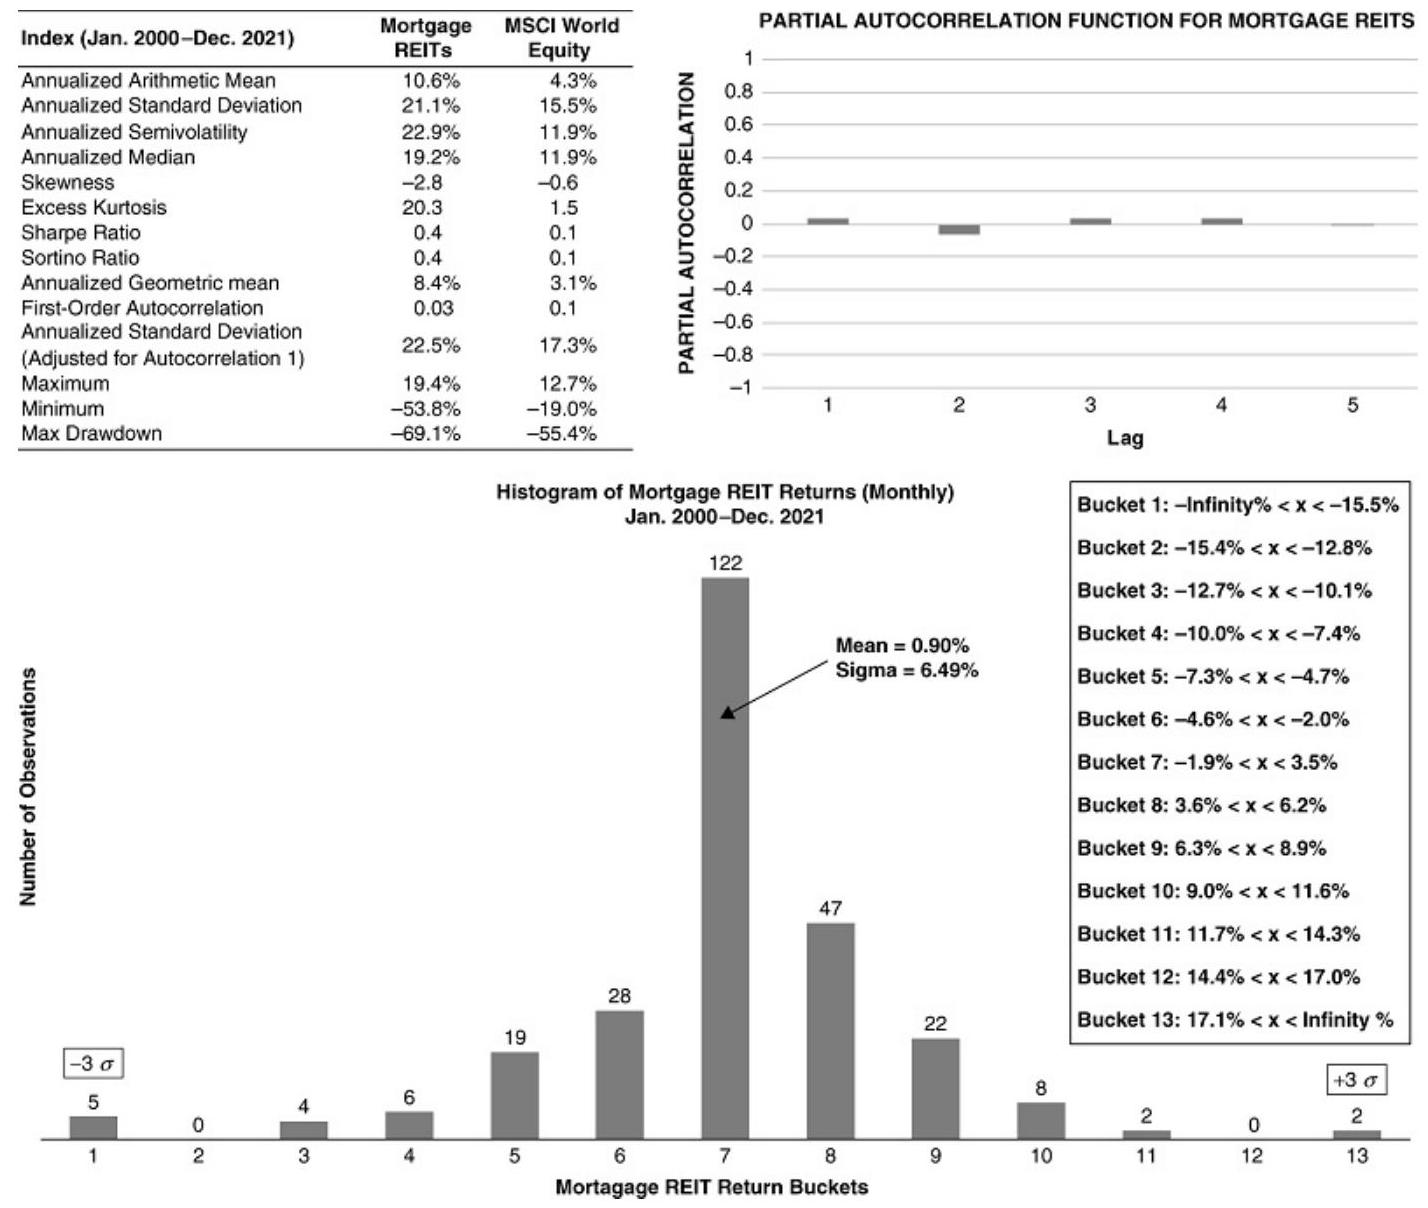
\includegraphics[max width=\textwidth]{2024_04_11_ce4a74e52a0c52a17383g-2}
\end{center}

Statistical Summary of Returns


\end{document}